\documentclass[11pt, letterpaper]{report}
\input{../../homework.tex}
\usepackage{titlepageBU}
\title{Honors Differential Equations}
\date{09/30/24}
\courseID{MA 231}
\courseSection{A1}
\begin{document}
\makeproblem
\section*{Section 1.6 Problem 6}
\begin{figure}[ht]
	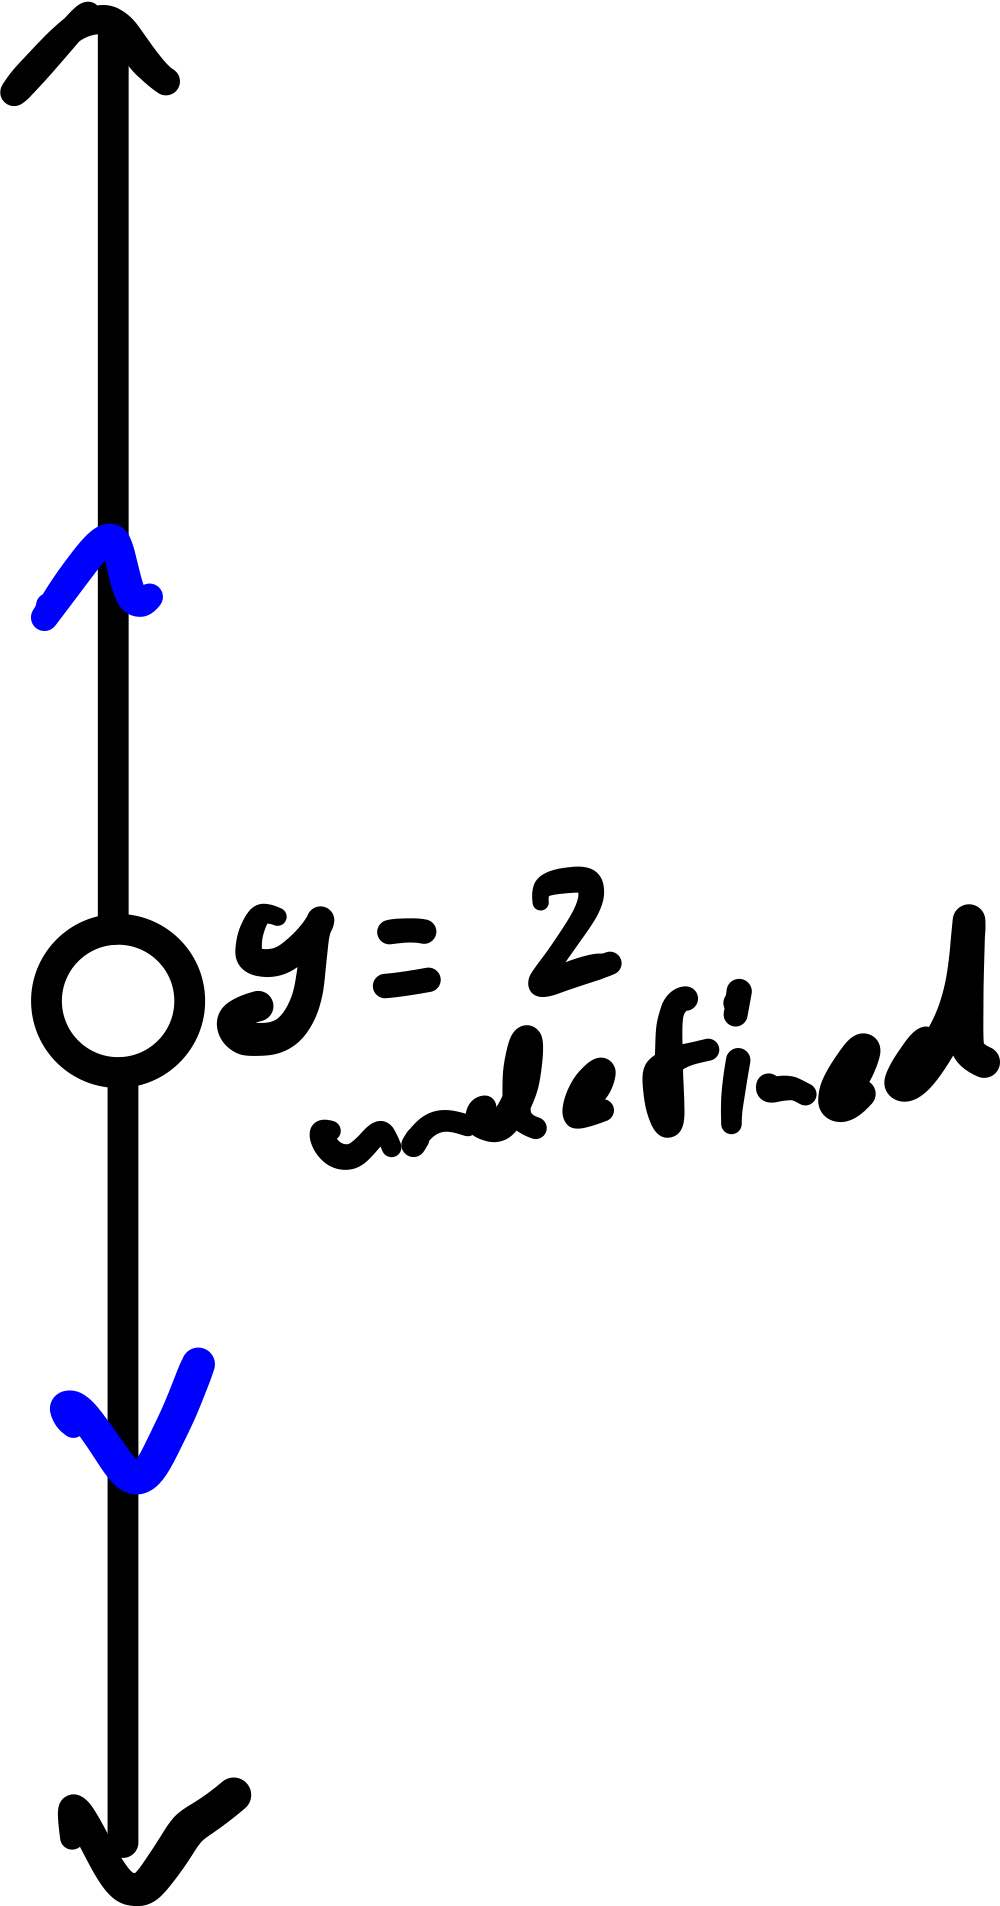
\includegraphics[scale=0.1]{phase1.jpg}
	\centering
\end{figure}
If we say the point where $\frac{\mathrm{d}y}{\mathrm{d}t} $ is undefined is an equilibrium point, then this point is a source. There are no other equilibrium points.
\section*{Section 1.6 Problem 8}
\begin{figure}[ht]
	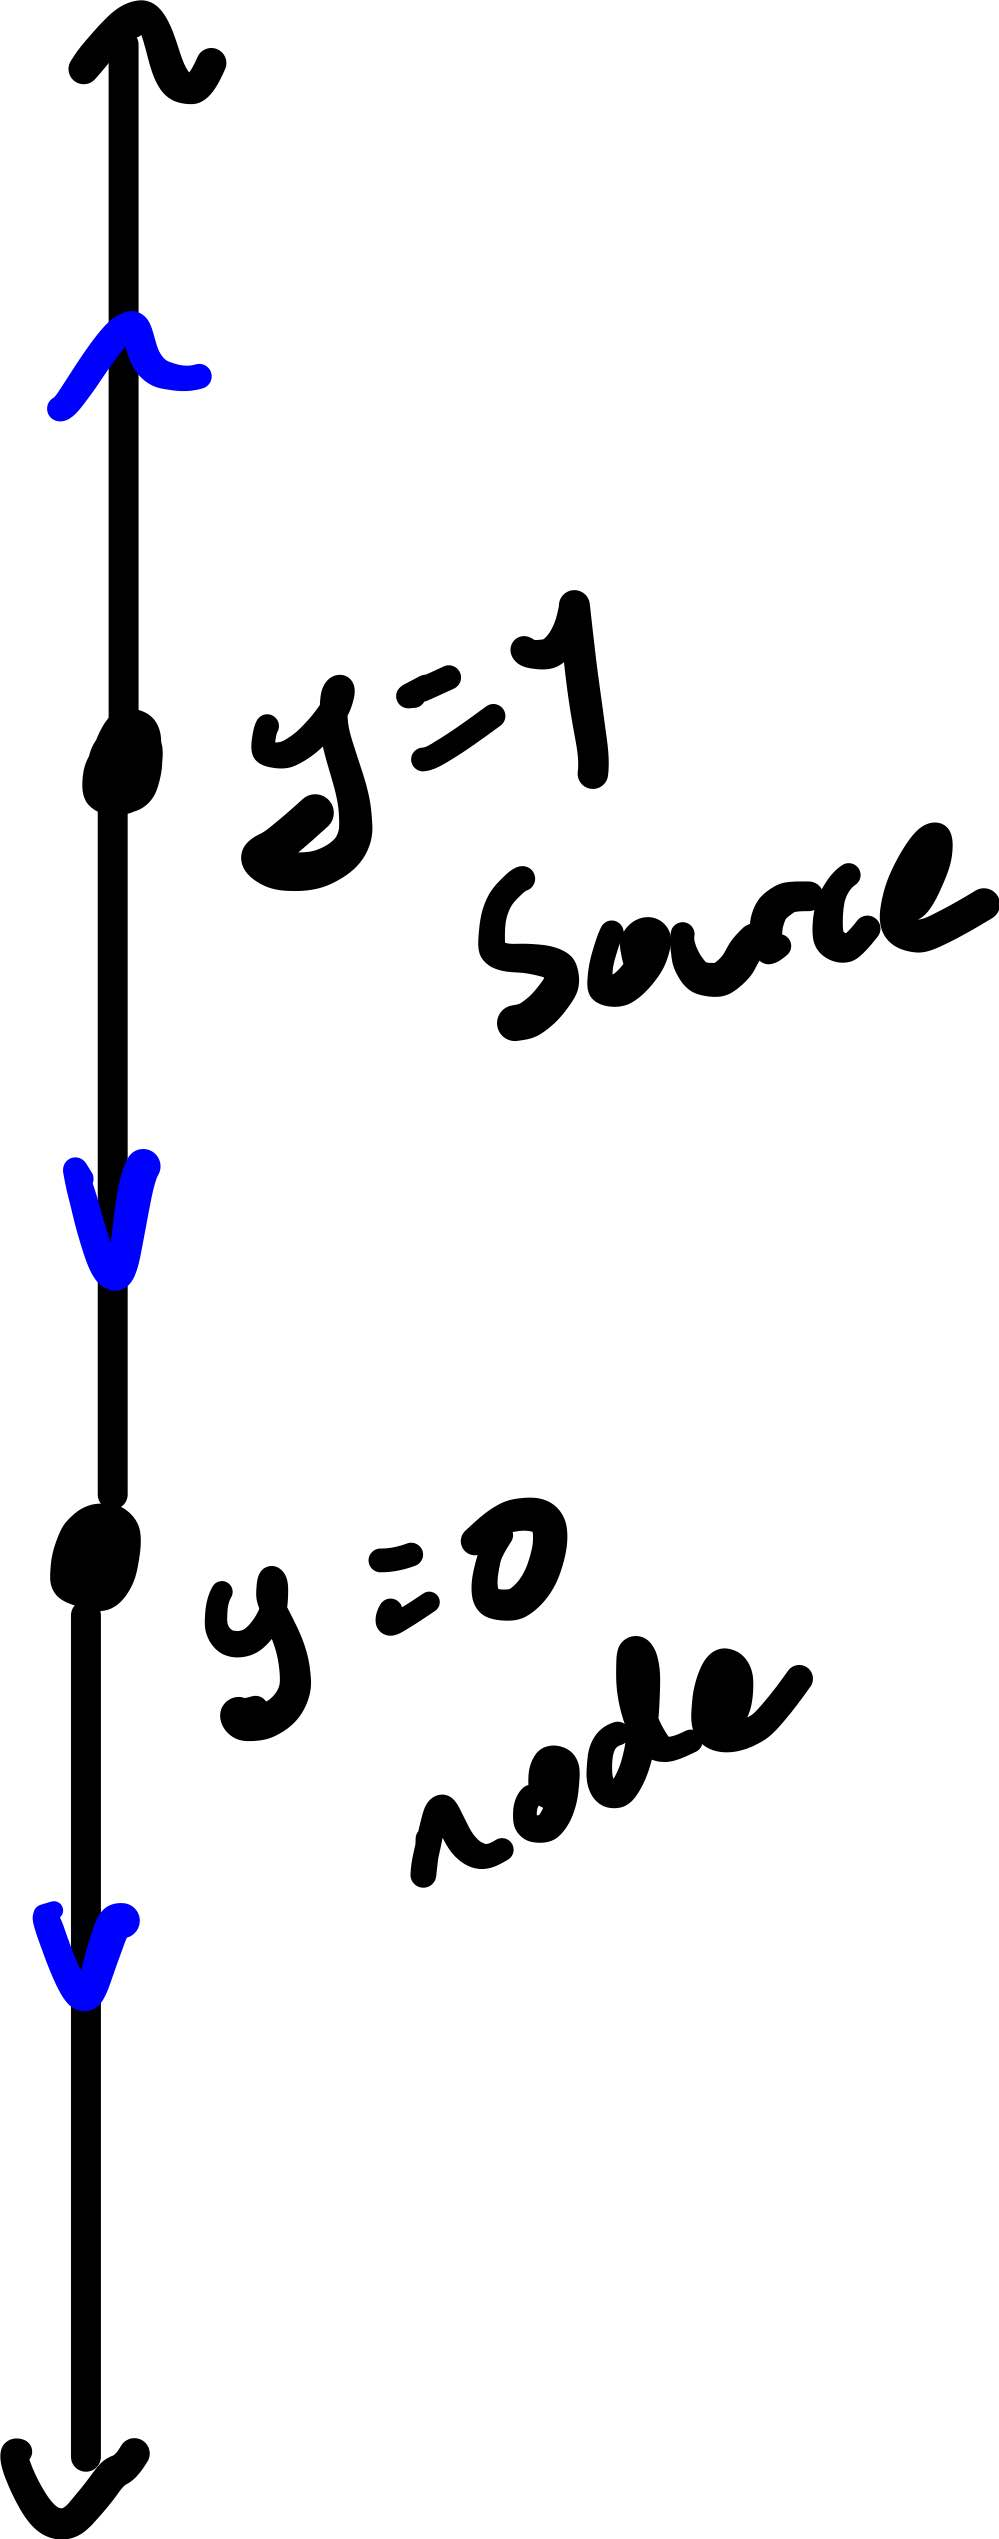
\includegraphics[scale=0.08]{phase2.jpg}
	\centering
\end{figure}
\section*{Section 1.6 Problem 28}
	We know that $y=-1$ and $y=2$ are equilibrium points. By Picard's theorem, no solutions can intersect, so for some initial value problem $y(0)=1$, we know that $-1<y<2$ for all values of $y$ and $t$. We then have two cases.

	\textbf{Case 1.} If there are no equilibrium points between $y=-1$ and $y=2$, then by the intermediate value theorem, $\frac{\mathrm{d}y}{\mathrm{d}t} $ will be either positive or negative for all $y\in(-1,2)$. Thus, $y(t)$ will either approach the equilibrium point $y=-1$ given a negative slope, or it will approach the equilibrium point $y=2$ given a positive slope.
\section*{Section 1.6 Problem 37}
	The equilibrium points for (ii), (iv), (vi), and (viii) all match those of (a) and (b). The phase line (a) gives $\frac{\mathrm{d}y}{\mathrm{d}t} >0$ for $y\in(0,1)$. Only (ii) and (viii) match this criteria. The phase line (a) also gives $\frac{\mathrm{d}y}{\mathrm{d}t} >0$ for $y<0$. For $y<0$, $y-y^2<0$. Therefore, (ii) does not go with the phase line, and thus (viii) goes with (a).

	This leaves (iv) and (vi) to consider for (b). The phase line (b) gives $\frac{\mathrm{d}y}{\mathrm{d}t} >0$ for $y<0$. Of the two, only (vi) satisfies this. Therefore, (vi) goes with (b).

	The equilibrium points for (i) match phase line (c). The only other function that might match (c) is (v), and (v) has no equilibrium point at 0. Therefore, (c) goes with (i).

The equilibrium points for both (iii) and (vii) match those of phase line (d). For $y\in(0,-1)$, the phase line gives a positive slope. On this interval, $\sin \left( \frac{\pi}{2}y \right) $ is negative. Since $\left| y \right| $ is always positive, and a positive times a negative is negative, (iii) cannot satisfy the phase line (d). Therefore, (vii) goes with (d).
\section*{Section 1.7 Problem 4}
The function has the bifrucation value $\alpha =0$. Notice that
\[
	f_\alpha (y)=y^2(y-\alpha )
.\]
For $f_\alpha =0$, we have the equilibrium points $y^2=0$ and $y=\alpha $. For  $\alpha <0$, the extra equilibrium point is at $y>0$. For $\alpha >0$, the extra point is at $y_0$. For $\alpha =0$, the point is at $y=0$, so all equilibrium points are at $y=0$.

\begin{figure}[ht]
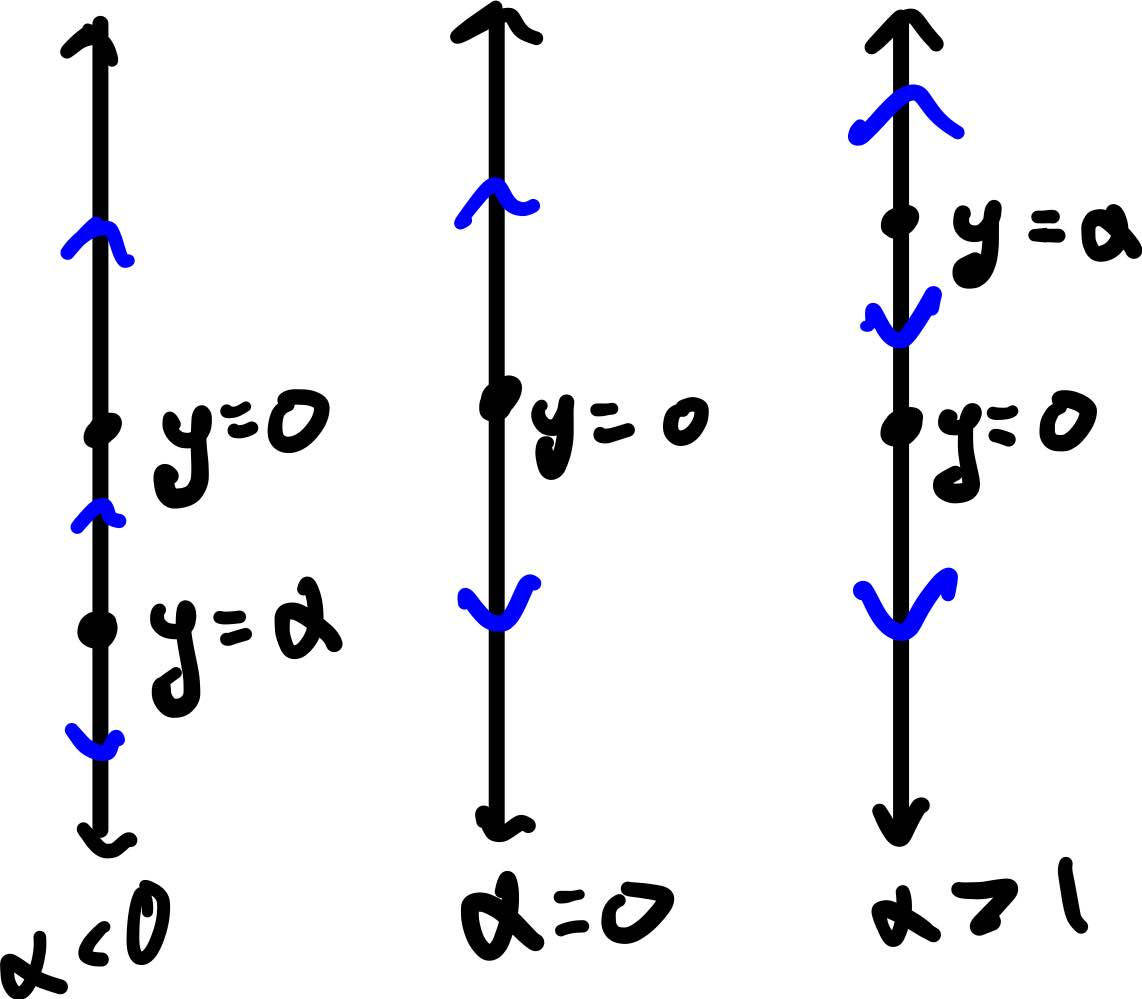
\includegraphics[scale=0.15]{phase3.jpg}
\centering
\end{figure}
\section*{Section 1.7 Problem 11}
Without loss of generality, we can assume the graph given has $\alpha =0$. At $\alpha=-2$, the equilibria that originally started at $y=0$ and $y\approx -2.4$ end up combining into a single equilibrium point. For $\alpha <-2$, the point disappears. Similarly, for $\alpha =2$, the points originally at $y=0$ and $y\approx 2.4$ combine into one, and for $\alpha >2$, the point disappears. Thus, the bifrucation values are $\alpha =\pm2$.
\section*{Section 1.7 Problem 13}
(iii) goes with (a). For all $A$, $y=0$ is an equilibrium point of (a). For $y=0$, we have
\[
	\frac{\mathrm{d}y}{\mathrm{d}t} =A(0)-0^3=0
,\]
which satisfies this property. For $y\neq 0$, (iii) has the equilibrium points
\[
	Ay-y^3=0\implies y=\pm \sqrt{A} 
,\]
which is what is seen in (a). There are no other functions with similar characteristics, so no further analysis is required.

(v) goes with (b). Let $\frac{\mathrm{d}y}{\mathrm{d}t} =0$. Then
\[
	y^2=A \implies y=\pm \sqrt{A} 
.\]
The function $y=\pm \sqrt{A} $ is precisely the function shown in (b). Additionally, in (b), $\frac{\mathrm{d}y}{\mathrm{d}t} >0$ for $A<0$. Take $A=-1$. We have
\[
	\frac{\mathrm{d}y}{\mathrm{d}t} =y^2-(-1)=y^2+1>0
.\]
Therefore, (v) goes with (b).

(iv) goes with (c). Similarly to (b), the graph is $y=\pm \sqrt{A} $, which are the equilibrium points of (iv). However, unlike (b), for $A<0$, $\frac{\mathrm{d}y}{\mathrm{d}t} <0$. Take $A=-1$ again. We have
\[
	\frac{\mathrm{d}y}{\mathrm{d}t} =-1-y^2<0
.\]
Therefore, (iv) goes with (c).

(i) goes with (d). For all $A$, $y=0$ is an equilibrium point of (d). For $y=0$, we have
\[
	\frac{\mathrm{d}y}{\mathrm{d}t} =A(0)-0^2=0
,\]
which satisfies this requirement. For $y\neq 0$, the other equilibrium point is
\[
	Ay-y^2=0 \implies y=A
.\]
This is what is shown in (d). The only other function sharing similar characteristics is (vi), but this gives $y=-A$, which is not what is seen in (d). Therefore, (i) goes with (d).

\section*{Section 1.8 Problem 3}
The solution to the associated homogeneous system is clearly $y=Ce^{-3t}$. Since we need a trig function as part of $y$, and $\sin $ and $\cos $ flip when we integrate them, we can \emph{guess} that the solution will be of the form
\[
	y=Ce^{-3t}+\alpha \sin (2t)+\beta \cos (2t)
.\]
Since the $Ce^{-3t}$ term is self contained, we only need to consider the other components of the equation. We know that
\[
\frac{\mathrm{d}}{\mathrm{d}t} \left( \alpha \sin (2t)+\beta \cos (2t) \right) =-3\left( \alpha \sin (2t)+\beta \cos (2t) \right) +4\cos (2t)
.\]
It follows that
\[
	\frac{\mathrm{d}}{\mathrm{d}t} \left( \alpha \sin (2t)+\beta \cos (2t) \right) =(4-3\beta )\cos (2t)-3\alpha \sin (2t)
.\]
Integrating both sides with respect to $t$, we obtain
\[
	\alpha \sin (2t)+\beta \cos (2t)=\int \left( 4-3\beta  \right) \cos (2t)-3\sin (2t) \,\mathrm{d} t=\frac{4-3\beta }{2}\sin  (2t)+\frac{3\alpha }{2}\cos  (2t)
.\]
It follows that
\[
	\alpha =\frac{4-3\beta }{2},\qquad \beta =\frac{3\alpha }{2}
.\]
Solving the second equation for $\alpha $, we have
\[
	\alpha =\frac{4-3\beta }{2}=\frac{2\beta }{3}
.\]
Multiplying both sides by $3\cdot 2$, we have
\[
	12-9\beta =4\beta 
.\]
It follows that $13\beta =12$, and thus $\beta =\frac{12}{13}$. Solving for alpha, we have
\[
	\alpha =\frac{2}{3}\beta =\frac{2}{3}\cdot \frac{12}{13}=\frac{8}{13}
.\]
Therefore,
\[
	y=Ce^{-3t}+\frac{8}{13}\sin (2t)+\frac{12}{13}\cos (2t)
\]
is the general solution to this equation.
\section*{Section 1.8 Problem 8}
The solution to the associated homogeneous equation is $y=Ce^{2t}$. Since the general solution will be of the form
\[
	y=Ce^{2t}+b(t)
,\]
where
\[
	\frac{\mathrm{d}b(t)}{\mathrm{d}t}  t=2b(t)+3e^{-2t}	
,\]
we can hypothesize that $b(t)$ is of the form
\[
	b(t)=-\frac{A}{2}e^{-2t}
.\]
Since $b'(t)=Ae^{-2t}=2b(t)+3e^{-2t}$, we have
\[
	Ae^{-2t}=2\left( -\frac{A}{2}e^{-2t} \right) +3e^{-2t}=\left( 3-A \right) e^{-2t}
.\]
Thus, $A=3-A$, and it follows that $A=3/2$. Therefore,
\[
	y(t)=Ce^{2t}-\frac{3}{4}e^{-2t}
.\]
Now we solve for the initial value problem. Let $t=0$ and $y=10$. We have
\[
	10=C-\frac{3}{4}\implies C=\frac{43}{4}
.\]
Therefore,
\[
	y(t)=\frac{43}{4}e^{2t}-\frac{3}{4}e^{-2t}
.\]
\section*{Section 1.8 Problem 13}
This problem is very similar to my thought process on problem 3 from the same section.

(a) Let $y_p(t)=\alpha \cos 3t$. It follows that $y_p'(t)=-\alpha \sin (3t)$. We must then have
\[
	-\alpha \sin (3t)=-2\alpha \cos (3t)+\cos (3t)=(1-2\alpha )\cos (3t)
.\]
Although $\sin $ and $\cos $ differ only by phase, the amplitude of the function cannot shift the phase, so there won't exist a solution here.

(b) The reason the previous solution failed is because the derivative and original function both need $\cos $ terms, but taking the derivative of a $\cos $ term yields a $\sin $ term. To rectify this, we can have the original function have both $\cos $ and $\sin $ terms, since the derivative of this will yield both $\cos $ and $\sin $ terms. Solving the problem then becomes an issue of identifying the amplitudes of the two terms, meaning our guess should be a function of the form
\[
	y_p(t)=\alpha \cos (3t)+\beta \sin (3t)
.\]
\newpage
\section*{Section 1.8 Problem 16}
\begin{figure}[ht]
	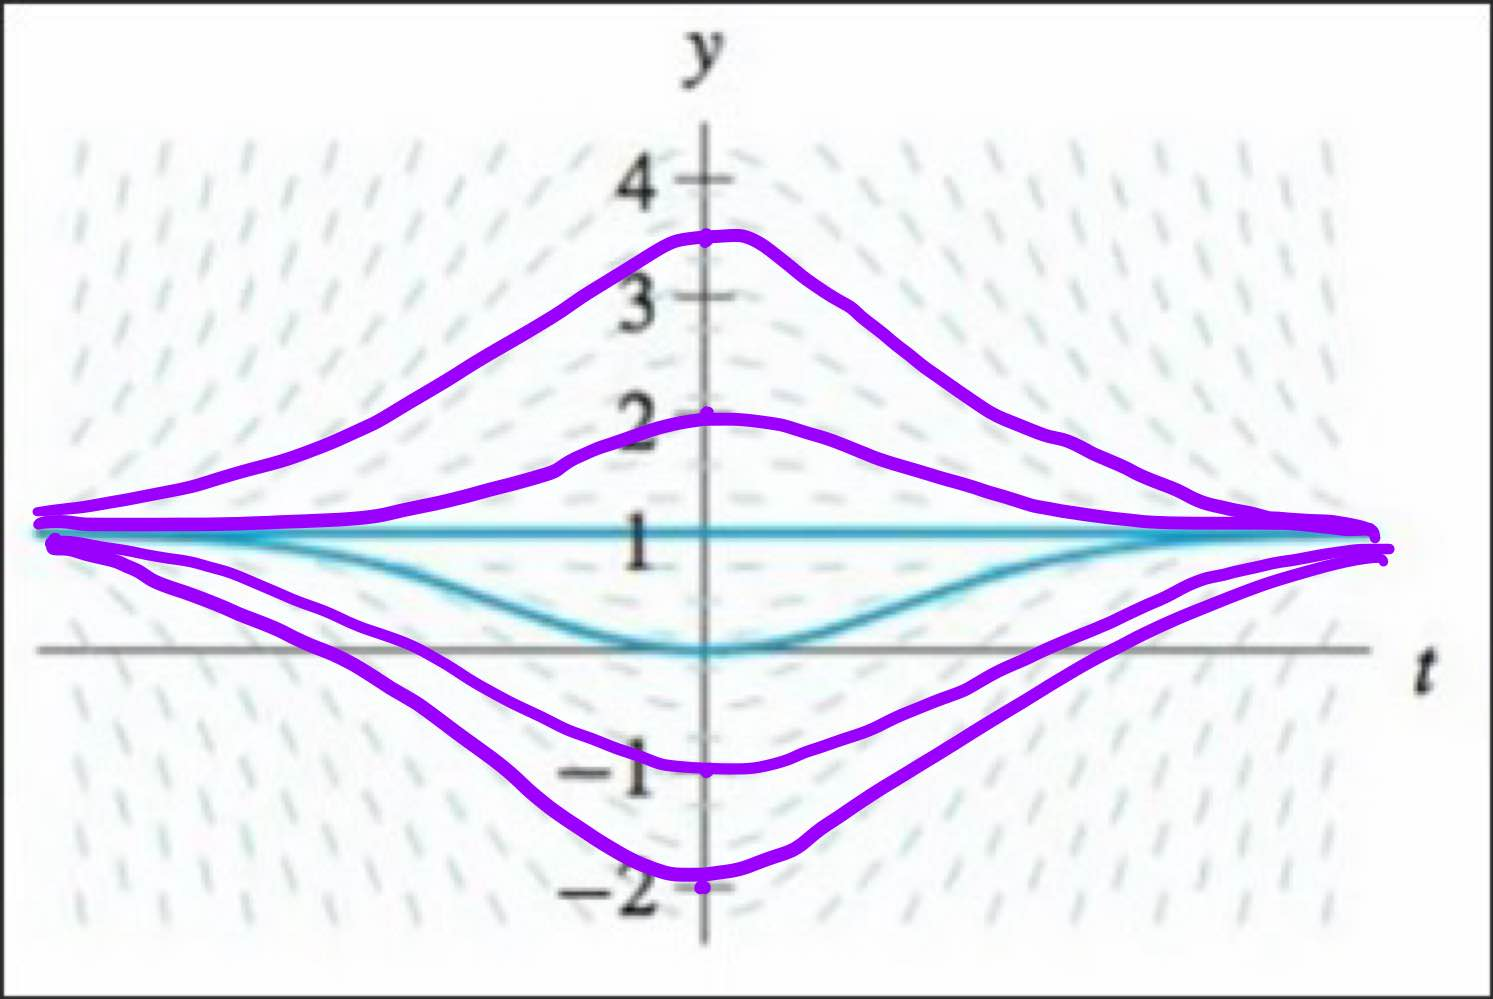
\includegraphics[scale=0.2]{phase4.jpg}
	\centering
\end{figure}
\section*{Supplimental 1}
\begin{proof}
	First, we establish some facts. Let $f$ have equilibrium point $y_1^*$ with no other equilibria in a neighborhood $[y_1^*-\delta ,y_1^*+\delta ]$. Let $a\in[y_1^*-\delta ,y_1^*)$ and $b\in(y_1^*,y_1^*+\delta ]$. Then by definition of a source, sink, and node, the following are true for all $a,b$:
	\begin{itemize}
		\item If $y_1^*$ is a source, then $f(a)<0$ and $f(b)>0$.
		\item If $y_1^*$ is a sink, then $f(a)>0$ and $f(b)<0$.
		\item If $y_1^*$ is a node, then both $f(a)$ and $f(b)$ are either less than or greater than zero.
	\end{itemize}
	This is all by definition; a source gives a negative slope for some $a<y_1^*$, and a positive slope for some $b>y_1^*$; a sink does the opposite; and a node has the same signs on both sides. Notice now that $i([a,b])=1$ implies $y_1^*$ is a source, and thus $f(a)<0$ and $f(b)>0$. Secondly, $i([a,b])=-1$ implies $y_1^*$ is a sink, and thus $f(a)>0$ and $f(b)<0$. Finally, $i([a,b])=0$ implies $y_1^*$ is a node, and thus either $f(a)$ and $f(b)$ are both positive, or they are both negative.

	Now suppose the proposition holds for an ordered set $\left\{ y^*_1, \dots, y^*_n  \right\} $ of equilibrium points. We must prove three cases.

	(a) Suppose for some $a<y_1^*,b>y_n^*$ that $f(a)<0$ and $f(b)>0$ for $n$ equilibrium points, and $i([a,b])=1$. Suppose there now exists a new equilibrium point $y_{n+1}^*>y_n^*$. This point cannot be a source, since a source requires $f(y_{n+1}^*-\delta )<0$ for $\delta <y_{n+1}^*-y_n^* $, but we know for any $b\in(y_n^*,y_{n+1}^*)$, we have $f(b)>0$. Therefore, $y_{n+1}^*$ can be only a node or a sink. This logic will be referenced again twice.

	Suppose now that $y_{n+1}^*$ is a node. Note that  $f(b)>0$, and by definition of a node, $f(c)>0$ for all $c>y_{n+1}^*$. We have the same overall signs of $f$, and $i([a,c])=i([a,b])+0=1$. Therefore, the proposition still holds.

	Suppose now that $y_{n+1}^*$ is a sink. Note that $f(b)>0$, and by definition of a sink, $f(c)<0$ for all $c>y_{n+1}^*$. We now have $f(a)<0$ and $f(c)<0$, but we now have $i([a,c])=i([a,b])-1=0$. Since both values of $f$ are negative and the index is 0, the proposition holds for case (a).

	(b) Suppose for some $a<y_1^*,b>y_n^*$ that $f(a)>0$ and $f(b)<0$ for $n$ equilibrium points, and $i([a,b])=-1$. Suppose there now exists a new equilibrium point $y_{n+1}^*>y_n^*$. By the same logic as in part (a), this point must be a source or a node.

	Suppose now that $y_{n+1}^*$ is a node. Note that $f(b)<0$, and by definition of a node, $f(c)<0$ for all $c>y_{n+1}^*$. We now have the same overall signs of  $f$, and $i([a,c])=i([a,b])+0=-1$. Therefore, the proposition holds.

	Suppose now that $y_{n+1}^*$ is a source. Note that $f(b)<0$, and by definition of a source, $f(c)>0$ for all $c>y_{n+1}^*$. We  now have $f(a)>0$ and $f(c)>0$, but we now have $i([a,c])=i([a,b])+1=0$. Since both values of $f$ are positive and the index is 0, the proposition holds for case (b).

	(c) Suppose for some $a<y_1^*,b>y_n^*$ that $f(a),f(b)>0$ or $f(a),f(b)>0$ for $n$ equilibrium points, and $i([a,b])=0$. Suppose there now exists a new equilibrium point $y_{n+1}^*>y_n^*$. By the same logic as in part (a), this point can be anything.

	Suppose now that $y_{n+1}^*$ is a node. If $f(b)>0$, then by definition of a node, $f(c)>0$ for all  $c>y_{n+1}^*$; and for $f(b)<0$, it also follows that $f(c)<0$. We have the same overall signs for $f$, and $i([a,c])=i([a,b])+0=0$. Therefore, the proposition holds.

	Suppose now that $y_{n+1}^*$ is a source, and thus $f(b)<0$. By definition of a source, $f(c)>0$ for all $c>y_{n+1}^*$. We now have $f(a)<0$ and $f(c)> 0$, but $i([a,c])=i([a,b])+1=1$. Therefore, the proposition still holds.

	Suppose now that $y_{n+1}^*$ is a sink. By the same logic as previously, $f(a)>0$ and $f(c)<0$ for all $c>y_{n+1}^*$. Since $i([a,c])=-1$, the proposition holds for case (c).

	By the method of induction, the proposition holds for equations of this class with finitely many equilibrium points.
\end{proof}
\section*{Supplimental 2}
\begin{center}
\begin{tabular}{ccc}
	\toprule
	$y_1^*$ &$y-2^*$ &$y_3^*$ \\
	\midrule
	node&node&node\\
	source&sink&node\\
	source&node&sink\\
	sink&source&node\\
	sink&node&source\\
	node&sink&source\\
	node&source&sink\\
	\bottomrule
\end{tabular}
\end{center}
\section*{Supplimental 3}
For $y_1^*$ and $y_3^*$ sources and $y_2^*$ a node, and since no other equilibria exist on $[a,b]$, we have $i[a,b]=1+1+0=2$. By the given proposition, $i([a,b])\in \left\{ -1,0,1 \right\} $ for any $[a,b]$. This proposition holds because the question asks if thisis true for the case that Supplimental problem 1 asked us to prove the problem from. Since $2\notin \left\{ -1,0,1 \right\} $ it is not possible for this to happen.
\end{document}
